\documentclass[11pt,a4paper]{article}
\usepackage{fontspec}
\setmainfont{TeX Gyre Pagella}
\setsansfont{Carlito}
\setmonofont{DejaVu Sans Mono}
\usepackage[a4paper,top=2.4cm,bottom=2.4cm,left=2.3cm,right=2.3cm,
            headheight=34pt,headsep=14pt]{geometry}
\usepackage{graphicx}\usepackage{fancyhdr}\usepackage{caption}
\usepackage{titlesec}\usepackage{booktabs}\usepackage{xcolor}
\usepackage{enumitem}\usepackage{amsmath}\usepackage{parskip}
\usepackage[hidelinks]{hyperref}
\definecolor{good}{HTML}{157A3C}
\titleformat{\section}{\sffamily\large\bfseries}{\thesection}{0.8em}{}
\titleformat{\subsection}{\sffamily\normalsize\bfseries}{\thesubsection}{0.8em}{}
\captionsetup[figure]{labelfont={sf,bf},textfont=small,labelsep=space}
\pagestyle{fancy}\fancyhf{}
\fancyhead[L]{
\includegraphics[height=30pt]{weekly_figs/header_banner.png}}
\fancyfoot[L]{\sffamily\small Weekly Report}\fancyfoot[R]{\sffamily\small\thepage}
\renewcommand{\headrulewidth}{0pt}\setlength{\parindent}{0pt}
\begin{document}
\thispagestyle{empty}
\begin{center}
  
\includegraphics[height=62pt]{weekly_figs/logo_kaust_academy.jpg}\hspace{28pt}
  
\includegraphics[height=62pt]{weekly_figs/logo_kaust.jpg}
\end{center}
\vspace{18pt}
\begin{center}
  {\sffamily\bfseries\LARGE Weekly Report}\\[10pt]
  {\large Ali Alhulaimi}\\[3pt]{\ttfamily\small alialhulaimi2005@gmail.com}
\end{center}
\vspace{16pt}
\begin{center}\begin{minipage}{0.88\linewidth}
{\sffamily\bfseries\large Abstract}\\[4pt]\small
This week I continued the work on fine-tuning the model using LoRA, this time using a dataset of 900 samples of SLats instead of the 300 used in the previous run, and raising the amount of training to six full passes over that data. Alongside the training work, we held a workshop in the FabLab about 3D clay printing. I helped the FabLab staff run a special clay printer, and I wrote G-code by hand to create different geometries on it. I also made a web interface that can slice 3D meshes based on the specific requirements of the clay printer, since clay does not tolerate the supports, overhangs and thin walls that a normal plastic slicer will happily produce. Finally, I discussed the possibility of further work on converting the model's outputs into clay-printable results, which is a different and stricter target than the plastic printing the validation layer was built for. This report covers that work, together with the fine-tuning, post-processing and web deployment work from the previous weeks, and the background material on the TRELLIS pipeline and on flow and diffusion models.
\end{minipage}\end{center}
\vspace{20pt}
\begin{center}\begin{minipage}{0.88\linewidth}\small
\begin{tabular}{@{}p{2.2cm}l@{}}
\textbf{Date:} & August 2026\\[3pt]
\textbf{Explainer:} & {\ttfamily\footnotesize\url{https://claude.ai/public/artifacts/c52594ab-8c5c-404c-8999-68e62b4054ee}}\\[3pt]
\textbf{Service:} & {\ttfamily\footnotesize\url{https://scifablabs-mac-mini.tailfc1a5e.ts.net/}}\\
\end{tabular}
\end{minipage}\end{center}
\newpage
\tableofcontents
\newpage


\section{Introduction}
\subsection{Overview}
This report covers the topics I have worked through over the past few weeks while preparing for the TRELLIS project: the TRELLIS pipeline itself and the flow/diffusion theory that TRELLIS is built on, along with my work running the model, post-processing its output, and --- this week --- putting it behind a web front end so that it can be used in the FabLab.

\subsection{Report Roadmap}
Section 2 lists the sources I studied over these past weeks. Section 3 summarizes the topics themselves, one subsection per topic. Section 4 covers my initial results, including the validation layer I built to make the model's output printable, together with the printed output and photos. Section 5 covers the deployment of the pipeline as a web service for FabLab use. Sections 6 to 8 cover the model-side work: extending the post-processing layer, an attempt at preference optimization, and fine-tuning the SLat flow model with LoRA, including this week's larger 900-sample run. Section 9 covers this week's FabLab clay printing workshop, the G-code and geometries I made for the clay printer, the web interface I built to slice meshes for it, and what converting the model's outputs into clay-printable results would involve. Section 10 is a short discussion, Section 11 covers limitations and next steps, and Section 12 concludes.


\section{Related Work}
The material I studied over the past few weeks comes from the MIT 6.S184 lecture notes on flow and diffusion models, and the TRELLIS and TRELLIS-2 papers on structured 3D latents, along with the DINOv3 paper referenced as an image feature extractor. This week I also read the TriFlow paper on generating artist-like 3D models and the DreamDPO work on preference optimization for diffusion models, and used the Thingi10K dataset for fine-tuning. Full citations are in the References section.


\section{Topics Covered Over the Past Few Weeks}
\subsection{TRELLIS Pipeline Overview}
I reviewed how the TRELLIS pipeline works end to end. Training data comes from three datasets. A 2D vision model (DinoV2) extracts visual features, while a voxelize step extracts spatial features. Both sets of features get a positional embedding and are passed into a VAE encoder, which produces a structured latent (SLat). The SLat then gets another positional embedding and is passed into a VAE decoder to reconstruct the output. This encoder-decoder setup is a variational autoencoder.

TRELLIS uses rectified flow transformers instead of regular transformers. Regular transformers predict the next token, but rectified flow transformers predict a continuous value instead, such as geometry, color, or texture. TRELLIS also uses time-adaptive normalization, and its tokens are made up of voxels and image patches. An interactive explainer of how this pipeline works is available online [5]; Figure 1 shows its stage-by-stage overview.

\begin{figure}[htbp]
  \centering
  
\includegraphics[width=\linewidth]{weekly_figs/fig1_pipeline.jpg}
  \caption{The five stages of the TRELLIS-2 image-to-3D pipeline, from DINOv3 image features through to the final PBR mesh, with the tensor shape handed between stages. Captured from the interactive explainer [5].}
\end{figure}
\subsection{Foundations of Flow and Diffusion Models}
I reviewed the general theory behind flow and diffusion models from the MIT lecture notes. Generation is framed as representing objects as vectors, for example images, videos, or molecular structures, each living in their own vector space. The data distribution is the distribution of objects we want to generate, and generating an object means sampling from it. The initial distribution is usually a standard Gaussian.

A flow model depends on an ordinary differential equation (ODE). A trajectory evolves over time according to a vector field, which assigns a direction to every point in time:

\[ \text{d/dt  X t  =  u t ( X t ).} \]
In practice this ODE is simulated step by step using the Euler method, starting from an initial point and repeatedly taking small steps in the direction of the vector field.

\subsection{Flow Matching}
Flow matching is how a flow model is actually trained. The goal is to learn a vector field u t theta, using a neural network, so that simulating its ODE moves samples from the initial (noise) distribution to the data distribution. Since the true target vector field can't be computed directly, training instead uses the conditional flow matching loss,

\[ \text{L CFM ( theta )  =  E [ || u t theta ( x ) --- u t target ( x | z ) || \textasciicircum{}2 ],} \]
which turns out to have the same gradient as the loss we actually want to minimize. Training samples a data point, a random time, and some noise, combines them into a single point along the path between noise and data, and updates the network to match the target direction at that point. The interactive explainer (Figure 2) visualizes this as draining a pool of noise into structure.

\begin{figure}[htbp]
  \centering
  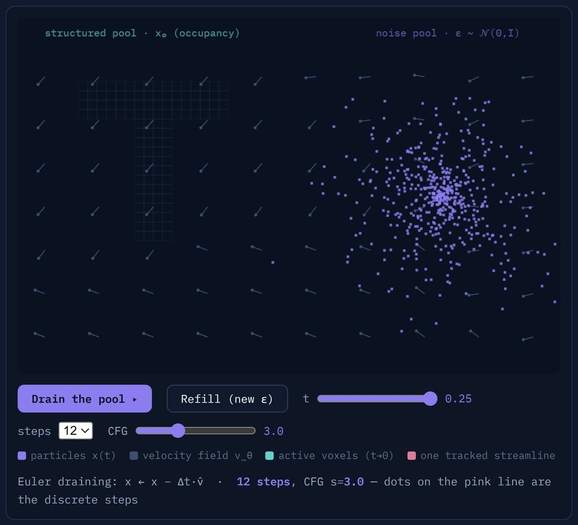
\includegraphics[width=0.85\linewidth]{weekly_figs/fig2_flowmatching.jpg}
  \caption{Flow matching shown as a ''pool'' analogy in the interactive explainer [5]: a learned velocity field carries particles from a pool of Gaussian noise (right) toward the structured voxel occupancy of the object (left, the T-shape), integrated with Euler steps at inference. The live version is interactive; a static view is shown here.}
\end{figure}
\subsection{Classifier and Classifier-Free Guidance}
I then reviewed guidance, which is how prompts get incorporated into generation. An unguided model just generates an image; a guided model generates, for example, ''an image of a cat'' given a prompt. Classifier guidance combines the unguided vector field with the gradient of a separately trained classifier. Classifier-free guidance (CFG) avoids training that separate classifier by instead combining a guided and an unguided vector field directly:

\[ \text{u\textasciitilde{} t w ( x | y )  =  w u t target ( x | y ) + (1 --- w) u t target ( x ),    w >= 1,} \]
where w controls how strongly the prompt is enforced, and the unguided term is just the same network run with an empty prompt. Bayes' theorem provides the background for this derivation.

\subsection{Latent Spaces and Variational Autoencoders}
I also looked at latent spaces and variational autoencoders (VAEs), which is how flow and diffusion models are made to work on compressed representations instead of raw data. A VAE encodes data into a distribution over a smaller latent space and decodes it back, trained with a loss that balances two goals: reconstructing the original data well, and keeping the latent distribution close to a standard Gaussian (measured with the KL divergence). This also includes the reparameterization trick, which makes it possible to backpropagate through the random sampling step, and the full beta-VAE training algorithm.

\subsection{Latent Diffusion Models and Transformer Architecture}
With VAEs covered, I looked at how latent diffusion models (LDMs) put everything together: take all the data, encode it into latents with a VAE, train a diffusion/flow model on this smaller latent dataset, and decode samples back to the original, uncompressed format after sampling. A concrete example of the size reduction this gives is an image going from shape [3, 256, 256] down to a latent of shape [4, 32, 32].

I also reviewed the neural network architecture used to implement the guided vector field: time is encoded with a sinusoidal embedding, the prompt is encoded with a pretrained language or image model (CLIP for text, or DINOv3 for image prompts, as used in 3D generation), and the latent image is split into patches. These three embeddings are combined inside a Diffusion Transformer (DiT), which uses self-attention over the image and cross-attention to bring in the prompt, with a time-adaptive layer norm to bring in the time information. As a case study, I looked at Stable Diffusion 3: a flow matching model with a straight-line scheduler, classifier-free guidance, and about 8 billion parameters, trained on the LAION dataset.


\section{Results}
Alongside the background reading above, I have also been running the TRELLIS model over the past few weeks. The model's raw output was not directly usable, so I built a validation layer that post-processes the model's output to make it printable. Photos of the printed output are shown below.

\begin{figure}[htbp]
  \centering
  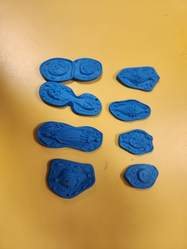
\includegraphics[width=0.23\linewidth]{weekly_figs/fig3_prints_a.jpg}\hfill
  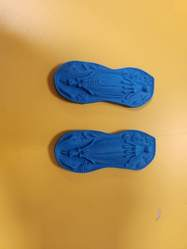
\includegraphics[width=0.23\linewidth]{weekly_figs/fig3_prints_b.jpg}\hfill
  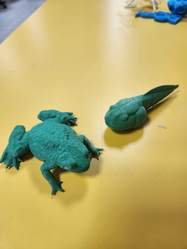
\includegraphics[width=0.23\linewidth]{weekly_figs/fig3_prints_c.jpg}\hfill
  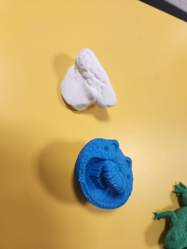
\includegraphics[width=0.23\linewidth]{weekly_figs/fig3_prints_d.jpg}
  \caption{Physical 3D prints of TRELLIS-generated models after post-processing through the validation layer. The validation layer repairs the model's raw output into a watertight, printable mesh.}
\end{figure}

\section{Web Deployment for FabLab Use}
\subsection{Motivation}
The main work this week was moving the model off my local command line and onto a web service so that it can actually be used in the FabLab. Running TRELLIS directly requires a GPU environment, the model weights, and a manual call to the validation layer described in Section 4. None of that is reasonable to ask of a FabLab user who simply wants a printable model from a photograph, so I wrapped the whole pipeline behind a web front end, SOLIDIFY, served from the lab machine.

\subsection{SOLIDIFY: Photo In, Mesh Out}
The interface follows the pipeline in one direction. The user supplies a single 2D photograph, the server runs the TRELLIS image-to-3D pipeline on it, the raw mesh is passed through the validation layer, and what comes back is a watertight STL that can be sent straight to the slicer. The intermediate representations discussed in Section 3 --- image features, the sparse structure, the structured latent --- are all hidden from the user; from the outside the site takes a photo in and gives matter out.

Figure 4 shows a field test through the deployed service. On the left is the input: a single phone photo of a frog figurine, with no turntable, scan rig, or multi-view capture. On the right is the mesh the lab machine reconstructed from that one image, checked as watertight and exported as STL. The green frog in Figure 3 is a print of this same kind of output, so the loop from photograph to physical object now runs end to end through the browser.

\begin{figure}[htbp]
  \centering
  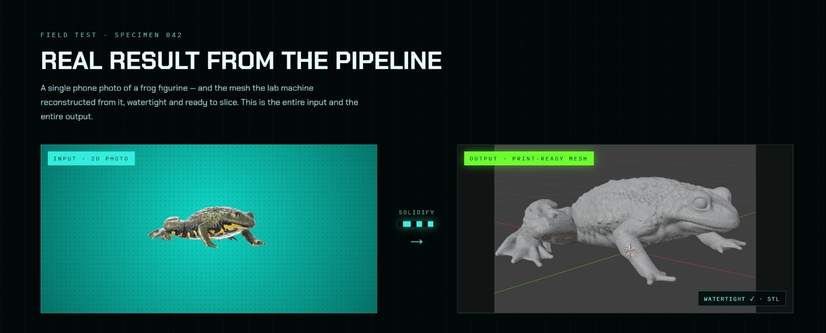
\includegraphics[width=\linewidth]{weekly_figs/fig4_solidify.jpg}
  \caption{The deployed SOLIDIFY front end showing a single field test: the input 2D photograph of a frog figurine (left) and the print-ready mesh reconstructed from it by the lab machine (right), flagged as watertight and exported as STL. Screenshot taken from the running service.}
\end{figure}
\subsection{Hosting}
The service runs on the lab Mac mini and is reached over the lab's private network rather than the public internet. This keeps the GPU and the model weights inside the lab while still letting any machine in the FabLab open the front end in a browser and submit a photo.


\section{Extending the Post-Processing Layer}
\subsection{Post-Processing Libraries and manifold3d}
Having the validation layer in place, I spent time this period trying to make it better. I tried many post-processing libraries and methods to improve the quality and printability of the model's output, adding different options for post-processing so that they could be compared on the same meshes. Of everything I tried, manifold3d [7] was the best for 3D printing, so I added it to the pipeline. I kept the original trimesh pipeline as well rather than replacing it, so both paths remain available.

\subsection{Reducing Non-Manifold Edges}
I also did further research on the best way to decrease the number of non-manifold edges in the models, since non-manifold edges are one of the defects that make a raw mesh awkward to slice. As part of that reading I went through the TriFlow paper on generating artist-like 3D models [8], which approaches mesh quality from the generation side rather than the repair side.

That distinction is what motivated the rest of this week's work. Post-processing can only repair what the model produces; it cannot change what the model tends to produce in the first place. The next two sections cover two attempts at improving the output at the source.


\section{Preference Optimization with DreamDPO}
The first attempt was to integrate DreamDPO [9] concepts into the pipeline. I read the DreamDPO work on preference optimization for diffusion models, which builds pairs of candidates during generation, has a ranking model say which one is preferred, and uses that preference to steer the optimization.

Rather than using a VLM as the ranking model, I simulated the preference discriminator as a score. This did not work. The results showed no gains, and the discriminator always chose the reference path for the flow model, so the preference signal never actually moved generation away from what the model would have produced anyway. Combined with my lack of expertise in this area of the theory, I set this approach aside rather than continuing to tune it.


\section{Fine-Tuning the SLat Flow Model with LoRA}
The second attempt was to fine-tune the SLat flow model directly, using LoRA methods, so that the improvement is in the model weights rather than in a steering step at generation time.

\subsection{Dataset}
I tried this on a small sample size of 300 curated 3D models from the Thingi10K dataset [10]. Thingi10K is a collection of real 3D-printing models from Thingiverse, and curation mattered: a large part of the collection has mesh defects of exactly the kind the fine-tuning is meant to reduce, so the 300 models were filtered to clean, closed, manifold meshes before being encoded into latents for training.

\subsection{Training and Results}
Initial training showed gains. The clearest result was on non-manifold edges: the fine-tuned model produced significantly less non-manifold edges for raw results --- that is, measured on the model's direct output, before manifold3d or the trimesh pipeline runs on it --- and this came without loss in detail.

How the metrics were measured. All four numbers are computed directly on the mesh the model produces, with no repair, decimation or simplification applied first. This matters: the same mesh measured after a simplification step reported a defect rate roughly fifty times higher, because simplification itself creates non-manifold edges, so any measurement taken after it describes the simplification rather than the model.

Every triangle has three edges, so each edge in the mesh can be counted by how many triangles share it. An edge shared by exactly two triangles is an ordinary interior edge. The open edge rate is the fraction of edges belonging to only one triangle, which is a hole or a border. The non-manifold edge rate is the fraction of edges shared by three or more triangles, which is geometry folding back on itself in a way a slicer cannot interpret as a surface. Both are reported as a fraction of all edges rather than a raw count, so that meshes with different triangle counts can be compared to each other.

Separate components counts how many disconnected pieces the mesh is made of, found by walking the triangles and grouping any that share an edge. A clean single object should be one piece; a large count means the model has shed loose fragments around the main body.

Detail is measured as surface energy. For each vertex, the average position of the vertices directly joined to it is computed, and the distance from the vertex to that average is squared and summed over the whole mesh. A vertex sitting exactly at the average of its neighbours contributes nothing, so a flat or smoothed surface scores low, while sharp edges, creases and fine features score high. Reporting it alongside the printability numbers is what shows the improvement is not simply the model producing smoother, emptier shapes.

The comparison itself is paired. The base model and the fine-tuned model were each asked to produce the same held-out objects using the same starting noise, so the two runs differ only by the model and not by the random draw. Without this the numbers were unusable: two runs of the same base model, differing only in their random draw, disagreed by more than a third on some metrics, which is larger than the effect being measured.

\begin{table}[htbp]\centering\small
\begin{tabular}{@{}lrr@{}}\toprule
\textbf{Measured on raw output} & \textbf{Base model} & \textbf{Fine-tuned} \\ \midrule
Non-manifold edge rate & 1.68\% & \textcolor{good}{\textbf{0.31\%}} \\
Open edge rate & 0.96\% & \textcolor{good}{\textbf{0.51\%}} \\
Separate components & 2,350 & \textcolor{good}{\textbf{447}} \\
Detail & no loss --- slightly higher &  \\
\bottomrule\end{tabular}\end{table}
Because these gains are on the raw output, they are made before manifold3d and the trimesh pipeline run, not instead of them. Both stay in the pipeline. I am continuing to collect more latent data for training, since 300 models is a small sample and the amount of training data is the main limit on how far this can go.

\subsection{Scaling the Dataset to 900 Samples}
This week I continued the fine-tuning with a larger dataset. The previous run used 300 curated models; this one uses 900 samples of SLats, encoded from Thingi10K models filtered the same way as before to clean, closed, manifold meshes. Of the 900, 870 are used for training and 30 are held out so that the model is always measured on objects it has not been trained on.

The other change is the amount of training rather than the amount of data. The run makes six full passes over the 900 samples, which is 5,220 training steps, where the previous larger attempt had made less than one pass before it was stopped. That distinction turned out to matter: when the 300-sample model was compared against a model trained on a larger dataset but for a shorter time, the 300-sample model won, and the most likely reason is not the data but the number of passes over it --- 8.7 passes against 0.78. Six passes over 900 samples is the first run in this project that exceeds the exposure of the model that currently performs best, which is what makes it a fair test of whether more data continues to help.

The setup is otherwise unchanged from the previous run so that the comparison means something: LoRA at rank 16 applied to the attention and MLP projections of the flow model's transformer blocks, with the base weights frozen, AdamW, a learning rate that warms up and then decays on a cosine schedule, and conditioning dropout so that the unconditional branch the sampler needs does not drift. At the time of writing this report the run is still in progress, so this section reports the setup rather than the result; the measured numbers will follow in the next report.

A smaller control run was completed first, using 100 samples for the same six passes. Its held-out loss stayed flat across all six passes, moving by less than a quarter of a percent from beginning to end while the training loss fell by a factor of four. That is what fitting a training set too small to generalize from looks like, and it is the reason for moving to 900 rather than continuing at 100.


\section{FabLab Clay Printing Workshop}
\subsection{The Workshop and the Clay Printer}
This week the FabLab held a workshop about 3D clay printing, and I helped the FabLab staff run the special clay printer used for it. [[FILL: printer make and model, the date of the workshop, and who attended --- staff, students, public]]

Clay printing is the same idea as the plastic printing assumed everywhere else in this report, but almost none of the practical constraints carry over. Instead of melting a filament and letting it solidify on contact, the machine extrudes a soft paste through a wide nozzle from a pressurised cartridge, and the material stays soft after it is placed. Everything that makes clay difficult follows from that. The material cannot bridge a gap, so an overhang has to be self-supporting or it will sag. Support structures are not a real option, because a support printed in clay is as soft as the part it is supporting and cannot be cleanly removed afterwards. The nozzle is much wider than a plastic nozzle, so layers are thick and walls cannot be thin. Extrusion cannot be started and stopped cleanly the way a plastic printer retracts, so a toolpath that jumps around leaves marks and blobs, and a continuous spiral path is usually preferred. And because the whole part is still wet while it is being built, the lower layers carry the weight of everything above them, which limits how tall and how fast a piece can be printed.

\subsection{Writing G-code for Test Geometries}
I wrote G-code to create different geometries on the printer. [[FILL: which geometries --- for example cylinders, cones, twisted vases, lattice or wave-patterned walls --- and what each was testing]]

Writing the toolpath directly, rather than going through a general-purpose slicer, is a reasonable way to work with a clay printer. The machine's behaviour depends on the extrusion rate being matched to the speed the head is moving at, and on the path being continuous, and both of those are easier to control when the path is generated deliberately than when it is the by-product of a slicer built for a different process. Hand-written G-code also makes it straightforward to produce the kind of geometry clay is actually good at: shapes generated as a single continuous spiral, where the wall thickness and the rate of change of radius are chosen so that each layer is supported by the one beneath it.

\begin{figure}[htbp]
  \centering
  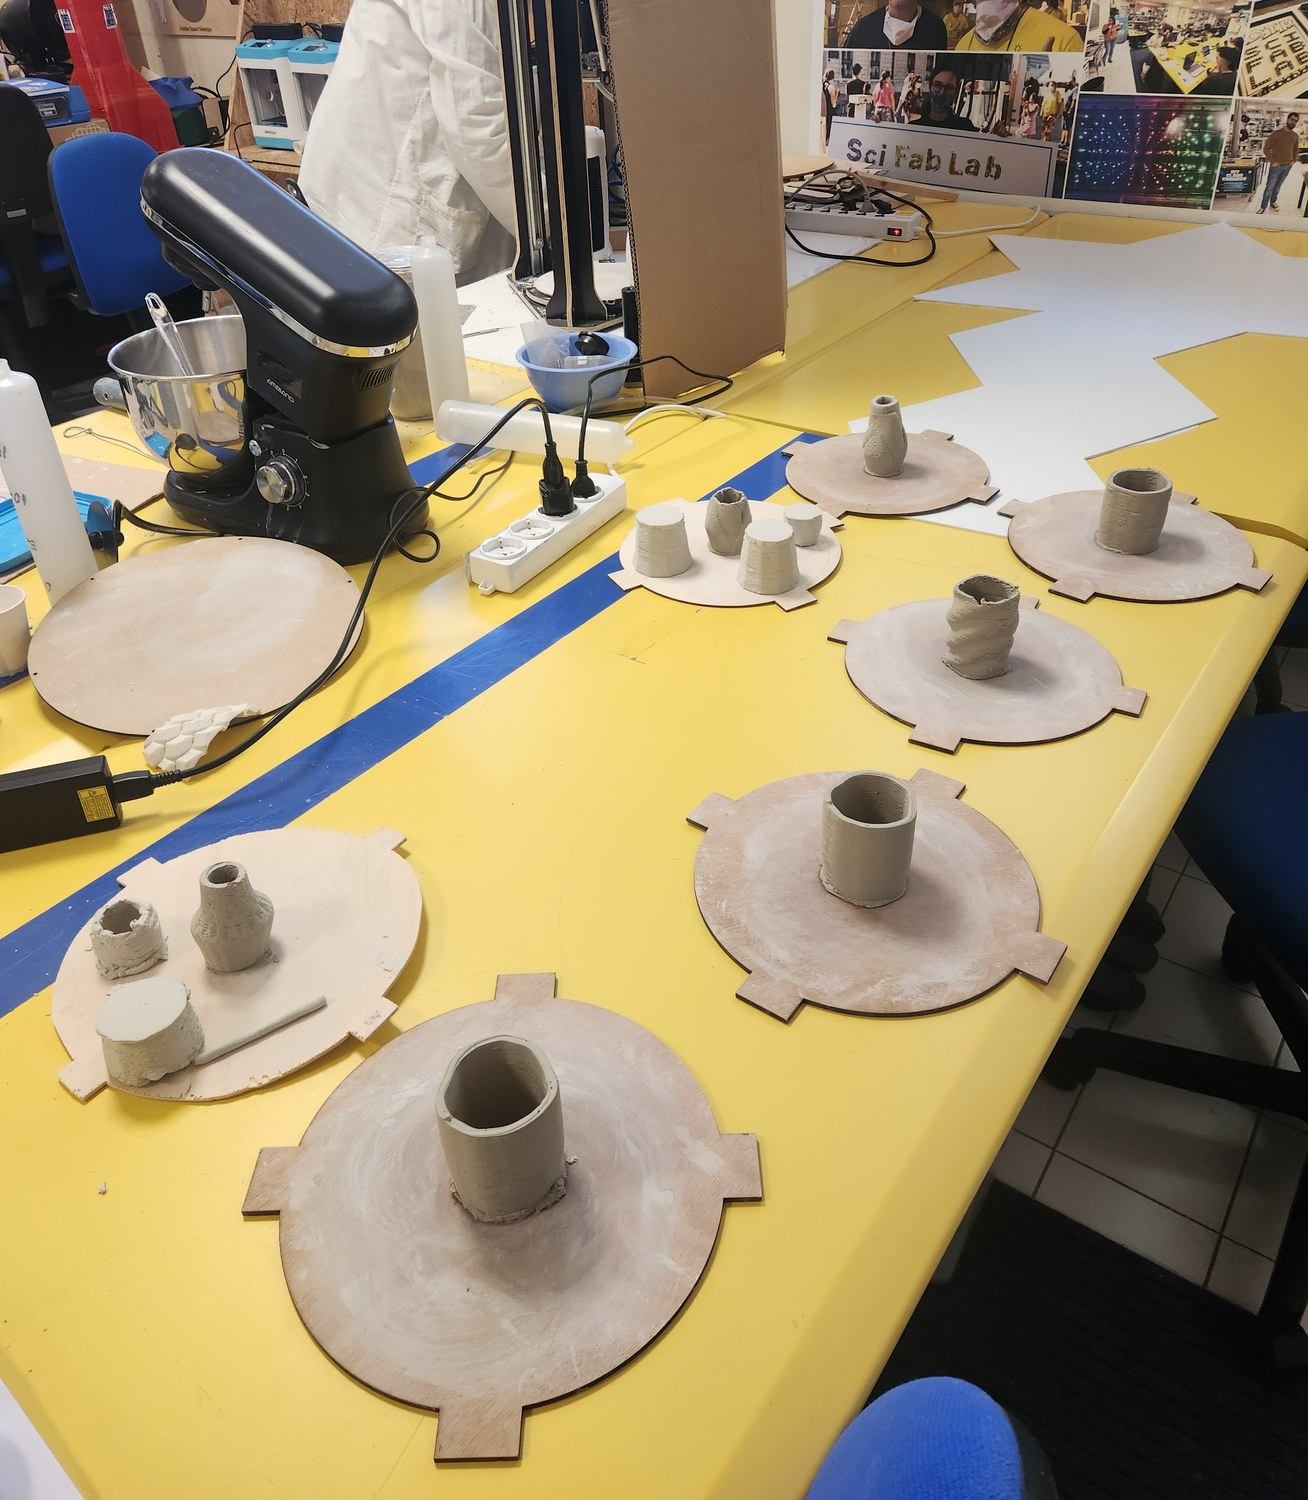
\includegraphics[width=0.46\linewidth]{weekly_figs/fig5_clay_table.jpg}\hfill
  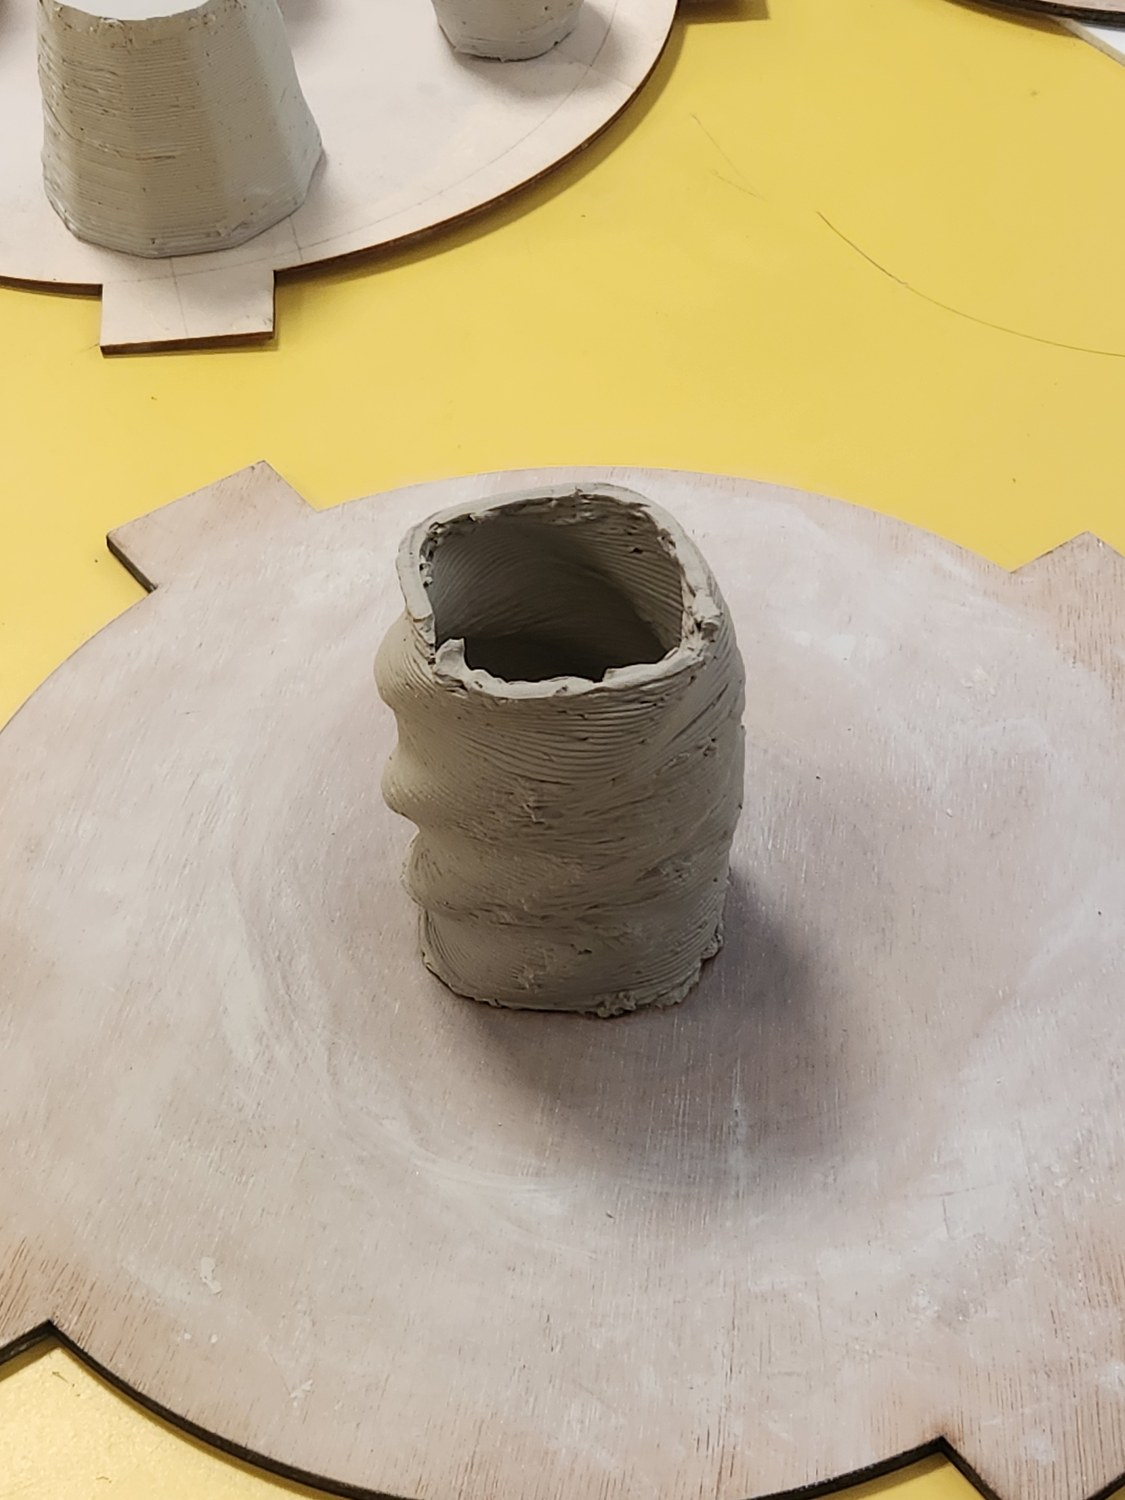
\includegraphics[width=0.46\linewidth]{weekly_figs/fig5_clay_piece.jpg}
  \caption{Pieces printed during the workshop. Left: the workbench, with each print left on its own laser-cut plywood bat so that it can be moved off the machine without being handled, and the clay mixer and the printer behind. The forms are cylinders, tapered cones and vessels of varying profile, printed as single continuous walls. Right: a close-up of one piece. The layer lines run as one unbroken spiral rather than as separate closed loops, and the lobed profile is produced by varying the radius as the spiral climbs, which is the kind of shape clay handles well because every layer stays supported by the one beneath it. The ragged top rim is where extrusion stopped.}
\end{figure}
\subsection{A Web Interface for Slicing to the Clay Printer}
I also made a web interface that can slice 3D meshes based on the specific requirements of the clay printer. The motivation is the same as for the SOLIDIFY front end described in Section 5: the knowledge of what the machine will and will not accept should live in the tool, not in the person operating it. A general slicer will happily generate supports, thin walls, sharp overhangs and a toolpath full of retractions, all of which are correct for plastic and wrong for clay, and it takes experience with the machine to know which of its settings to override.

The interface takes a mesh, applies the constraints the clay printer needs, and produces a toolpath the machine can run. [[FILL: what the interface is called, what it is built with, which parameters it exposes --- nozzle diameter, layer height, extrusion rate, maximum overhang angle, minimum wall thickness, spiral or shelled mode --- and whether it previews the toolpath before printing]]

[[FILL: add a screenshot of the interface here. Drop the image into report/weekly\_figs/ and it can be placed the same way as Figure 5.]]

\subsection{From Model Output to Clay-Printable Results}
Finally, I discussed the possibility of further work on converting the model's outputs into clay-printable results, so that the pipeline described in this report could end at the clay printer rather than at a plastic one.

This is a harder target than plastic, and the difference is instructive. For plastic, the validation layer's job is almost entirely repair: make the mesh closed and manifold so that the slicer will accept it, and the printer will handle the rest, using supports where the geometry needs them. For clay, a mesh can be perfectly closed and manifold and still be impossible to print, because the constraints are about the shape itself rather than about the correctness of the surface. Overhang angle, wall thickness and how much unsupported weight sits above a given layer are all properties of the geometry the model chose to generate, and no amount of repair after the fact will change them.

That is exactly the kind of property fine-tuning can reach, which is what makes this worth pursuing rather than treating as a separate problem. The scoring function already used to evaluate the fine-tuned models measures an overhang penalty and a thickness penalty alongside the mesh-quality metrics, because those were the axes expected to respond to training in the first place. A clay-specific version of that scoring, with the thresholds set by what the machine can actually do, would give a direct way to measure whether a model's raw output is clay-printable, and therefore a direct target to fine-tune towards. Whether the improvement would be large enough to matter is an open question, and answering it needs the clay constraints written down as numbers first. [[FILL: the printer's actual limits --- nozzle diameter, usable overhang angle, minimum wall thickness, maximum practical height]]


\section{Discussion}
The problem this period has really been about is not whether the model's output can be made printable, but whether it can be made printable while keeping the detail the model produced in the first place. Those two goals pull against each other. Repair works by changing the surface, and the more aggressively a method has to change the surface to close it up, the more of the original shape it loses along the way.

My first approach used trimesh. In terms of printability the results were good: it produced meshes that were closed and that a slicer would accept. In terms of preserving detail it was less good, and that is the trade-off in practice --- the repaired mesh was printable, but noticeably smoother and simpler than what the model had actually generated, so some of the fine features that made the output worth printing were gone by the time it reached the printer.

manifold3d did a better job on that second point. It reaches a printable result while changing the surface less, so more of the original detail survives the repair step, which is why I added it and kept it as the main path.

Both of those are still repairs applied after the fact, and a repair can only work with the mesh it is given. That is the reason for moving to fine-tuning: if the model's raw output starts out with fewer defects, then less repair is needed, and less repair means less detail is lost. The early fine-tuning results point that way --- fewer non-manifold edges and fewer loose fragments in the raw output, with the detail measurement slightly higher rather than lower --- and we hope that continued fine-tuning improves this aspect further, so that the repair step has less to undo.


\section{Limitations and Next Steps}
The main limitation is data. The fine-tuning was done on 300 curated models, which is a small sample for training a model of this size, and it is the clearest constraint on the result. It also means the numbers reported here should be read as an early indication rather than a settled figure: they come from a small held-out set, and a larger and more varied training set could move them in either direction.

The second limitation is that I do not yet know how much more improvement is available. The gains measured so far came from a first run on a small dataset, and there is no way to tell from that alone whether the remaining defects are something more training data would remove, or whether they come from a part of the pipeline that fine-tuning the flow model cannot reach at all. Until a larger run is done, how much headroom is left is an open question.

The next step is therefore to collect more latent data and train on it, and to see whether the improvement continues at the same rate, slows down, or stops. Alongside that I plan to keep testing the post-processing path on more model outputs, and to continue working through the flow and diffusion theory where the lecture notes currently leave off.


\section{Conclusion}
Over the past few weeks I reviewed the background theory behind TRELLIS: the TRELLIS pipeline itself and the flow matching, guidance, VAE, and transformer-architecture material from the MIT lecture notes. I also ran the model and built a validation layer to post-process its output into a printable form, with physical prints included above, and put that pipeline behind a web front end, SOLIDIFY, hosted on the lab machine, so that a FabLab user can upload a single photograph and get back a watertight, print-ready mesh. I extended the post-processing side with manifold3d, tried and set aside a DreamDPO-based preference approach, and fine-tuned the SLat flow model with LoRA on 300 curated Thingi10K models, which gave significantly less non-manifold edges on the raw output without loss in detail. This week I continued that fine-tuning with a larger dataset of 900 SLat samples trained for six full passes. Alongside the model work, we held a FabLab workshop on 3D clay printing, where I helped the staff run the clay printer, wrote G-code to produce different geometries, and built a web interface that slices meshes to the clay printer's specific requirements. Converting the model's outputs into clay-printable results is the direction I would like to take next, since clay constrains the shape itself rather than only the correctness of the mesh, and that is a constraint fine-tuning can be aimed at directly.

\section*{References}\addcontentsline{toc}{section}{References}
\begin{enumerate}[leftmargin=*,itemsep=3pt]
  \item P. Holderrieth and E. Erives. Introduction to Flow Matching and Diffusion Models. MIT 6.S184 course notes and lectures, 2026. \url{https://diffusion.csail.mit.edu/2026/}
  \item J. Xiang, Z. Lv, S. Xu, Y. Deng, R. Wang, B. Zhang, D. Chen, X. Tong, and J. Yang. Structured 3D Latents for Scalable and Versatile 3D Generation (TRELLIS). arXiv:2412.01506, 2024.
  \item J. Xiang, X. Chen, S. Xu, R. Wang, Z. Lv, Y. Deng, H. Zhu, Y. Dong, H. Zhao, N. J. Yuan, and J. Yang. Native and Compact Structured Latents for 3D Generation (TRELLIS-2). arXiv:2512.14692, 2025.
  \item O. Simeoni et al. DINOv3. arXiv:2508.10104, 2025.
  \item Interactive explainer: How TRELLIS-2 Works. \url{https://claude.ai/public/artifacts/c52594ab-8c5c-404c-8999-68e62b4054ee}
  \item SOLIDIFY web service (internal, lab network). \url{https://scifablabs-mac-mini.tailfc1a5e.ts.net/}
  \item Manifold3D --- mesh library for manifold geometry. \url{https://github.com/elalish/manifold}
  \item TriFlow --- paper on generating artist-like 3D models.
  \item Z. Zhou, X. Xia, F. Ma, H. Fan, Y. Yang, and T.-S. Chua. DreamDPO: Aligning Text-to-3D Generation with Human Preferences via Direct Preference Optimization. arXiv:2502.04370, 2025.
  \item Q. Zhou and A. Jacobson. Thingi10K: A Dataset of 10,000 3D-Printing Models. arXiv:1605.04797, 2016.
  \item Clay 3D printer used in the FabLab workshop. [[FILL: manufacturer, model, and a link to its documentation]]
  \item Clay slicing web interface (internal, lab network). [[FILL: name and URL if it is deployed]]
\end{enumerate}
\end{document}
